%%%%%%%%%%%%%%%%%%%%%%%%%%%%%%%%%%%%%%%%%%%%%%%%%%%%%%%%%%%%%%%%%%%%%%%%%%%%%%%%
\section{Appendix -- Community Connections}
{   
	\usebackgroundtemplate{
		\vbox to \paperheight{\vfil\hbox to \paperwidth{\hfil
\includegraphics[height=\paperheight]{up_to_date.jpg}\hfil}\vfil}
		%https://www.flaticon.com/free-icon/decoration_2788716
		%<a href="https://www.flaticon.com/free-icons/decoration" title="decoration icons">Decoration icons created by Freepik - Flaticon</a>
		
	}
	\frame{
		\frametitle{Keeping your Community Up to Date}
		\begin{mdframed}[tikzsetting={draw=white,fill=white,fill opacity=0.8,
				line width=0pt},backgroundcolor=none,leftmargin=0,
			rightmargin=150,innertopmargin=4pt,roundcorner=10pt]
			\tableofcontents[currentsection,sections={1-6},hideothersubsections]
		\end{mdframed}
	}
}

%%%%%%%%%%%%%%%%%%%%%%%%%%%%%%%%%%%%%%%%%%%%%%%%%%%%%%%%%%%%%%%%%%%%%%%%%%%%%%%%
\begin{frame}
	\frametitle{Automated Social Media Posts - here: Mastodon}
	\begin{columns}
		\begin{column}{0.4\textwidth}
			
\includegraphics[width=0.6\textwidth]{bot.jpg}
			\vfil
			\only<2>{
\includegraphics[width=0.5\textwidth]{qrcode.png}}
		\end{column}
		\begin{column}{0.6\textwidth}
			Example post:\\
			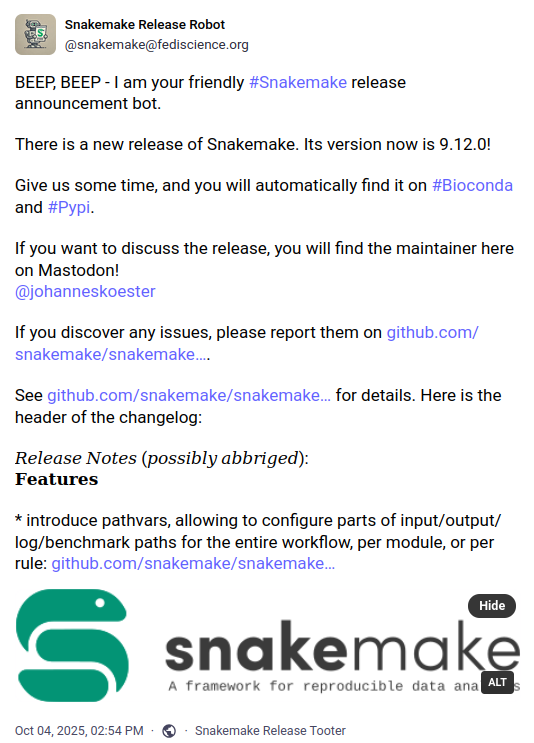
\includegraphics[width=0.55\textwidth]{snakemake_bot_post.png}
		\end{column}
	\end{columns}
\end{frame}

%%%%%%%%%%%%%%%%%%%%%%%%%%%%%%%%%%%%%%%%%%%%%%%%%%%%%%%%%%%%%%%%%%%%%%%%%%%%%%%%
\begin{frame}
	\frametitle{And if my Audience is not in the Fediverse?}
	Take a \lhref{https://github.com/defnull/fediwall}{fediwall} -- an appendix to a homepage, e.\,g.:
	
\end{frame}


%%%%%%%%%%%%%%%%%%%%%%%%%%%%%%%%%%%%%%%%%%%%%%%%%%%%%%%%%%%%%%%%%%%%%%%%%%%%%%%%
\begin{frame}[fragile]
	\frametitle{How does it work?}
	It uses a \lhref{https://github.com/snakemake/mastodon-release-post-action/}{special action}, key is the (Mastodon)-Secret:
	
			\begin{lstlisting}[language=yaml,basicstyle=\small\ttfamily\relax]
jobs:
  post_to_mastodon:
    if: "${{ contains(github.event.head_commit.message, 'chore(main): release') }}"
    runs-on: ubuntu-latest 
  steps: 
    - name: Checkout repository
      uses: actions/checkout@v4
    - name: Post to Mastodon
      uses: snakemake/mastodon-release-post-action@main 
      with:
        !access-token: ${{ secrets.MASTODONBOT }}!
		    \end{lstlisting}

\end{frame}